\documentclass[conference]{IEEEtran}
\IEEEoverridecommandlockouts
\usepackage{cite}
\usepackage{amsmath,amssymb}
\usepackage{graphicx}
\usepackage{booktabs}
\usepackage{multirow}
\usepackage{array}
\usepackage{xcolor}
\usepackage{tikz}
\usetikzlibrary{arrows.meta,positioning,shapes.geometric,fit,calc,automata}
\usepackage[hidelinks]{hyperref}
\graphicspath{{../docs/figures/}}


\begin{document}

\title{Design and FPGA Evaluation of a Parameterized Output-Stationary Systolic Array Accelerator for Fixed-Point Matrix Multiplication%
\thanks{Team DnD, Project 12, Modern Computer Architecture; B.Tech, Computer Science and Artificial Intelligence.}}

\author{\IEEEauthorblockN{Syed Darain Qamar, Md Sajjan, Sibtain Ahmed Qureshi, Abuzar Haideri, Antik Mondal}}

\maketitle

% ============================================================================
\begin{abstract}
Matrix multiplication dominates the run time of modern deep-learning
workloads, and dedicated systolic-array hardware such as Google's Tensor
Processing Unit (TPU) has become the standard way to accelerate it. This
paper presents the design, verification and field-programmable gate array
(FPGA) evaluation of a small, fully parameterized \emph{output-stationary}
systolic-array accelerator written in synthesizable Verilog. The design is
built bottom-up from a signed fixed-point multiply--accumulate (MAC) unit, a
processing element (PE) that forwards data to its neighbors, input buffers,
skew buffers, a grid of PEs, output registers and a finite-state machine (FSM)
controller behind a simple data interface. A pipelined-MAC variant and a
single-MAC sequential multiplier were also built for comparison.
Self-checking testbenches ran 224 matrix products (2\,800 result elements)
for 3-by-3 and 4-by-4 arrays, and every result matched both a Verilog
reference model and an independent NumPy model. One $N\times N$ product takes
exactly $3N+1$ clock cycles, against $N^2(N+1)+1$ for the sequential
baseline: a 6.2$\times$ cycle speed-up for $N=4$ that grows to
23.1$\times$ for $N=8$. After place-and-route on a Lattice ECP5, the 4-by-4
array runs at 100.5\,MHz, or 127.0\,MHz with the pipelined MAC, sustaining
1.16 giga-operations per second (GOPS) and a 7.9$\times$ wall-clock speed-up
over the baseline. On a Xilinx Artix-7 it uses 233 look-up tables (LUTs),
789 flip-flops and 16 DSP48E1 slices.
\end{abstract}

\begin{IEEEkeywords}
AI hardware, fixed-point, FPGA, hardware accelerator, matrix multiplication,
multiply--accumulate, processing element, systolic array, Verilog
\end{IEEEkeywords}

% ============================================================================
\section{Introduction}
General matrix multiplication (GEMM) $C = A\times B$ is the computational core
of fully-connected layers, convolutions (via im2col), attention, and many
signal-processing kernels. A naive implementation on a scalar processor
performs $N^3$ MAC operations one after another and is limited by the memory
bandwidth needed to fetch two operands per MAC. Systolic arrays, introduced by
Kung and Leiserson~\cite{kung1979systolic,kung1982why}, solve both problems:
a regular grid of simple PEs computes $N^2$ MACs per cycle, and each operand
fetched from memory is reused $N$ times as it is pumped from PE to PE through
short local wires. This principle underlies Google's Tensor Processing Unit
(TPU)~\cite{jouppi2017tpu}, whose $256\times256$ array delivers 92 tera-operations
per second (TOPS) of INT8 throughput.

This project translates those ideas, covered in the Modern Computer Architecture units on
parallelism, pipelining and modern AI hardware~\cite{hennessy2019ca}, into a
verified field-programmable gate array (FPGA) implementation. The
contributions are:
\begin{enumerate}\setlength{\itemsep}{1pt}
\item A modular, parameterized ($N$, operand width, accumulator width,
  pipelining) Verilog register-transfer level (RTL) description of an output-stationary systolic array with every
  sub-module requested by the project brief: MAC unit, PE, input buffers,
  output/accumulator registers, systolic controller and matrix data interface.
\item A closed-form, cycle-exact latency model ($3N+1$ cycles) that is
  confirmed by simulation, and a proof that the controller's drain time is
  minimal.
\item A directed and randomized self-checking verification environment with
  an independent NumPy golden model and waveform analysis.
\item Synthesis, place-and-route and timing results for two FPGA families and a
  quantitative comparison against a sequential single-MAC baseline and a
  pipelined-MAC alternative.
\item A ready-to-program Basys-3 demonstration wrapper for live demonstration.
\end{enumerate}

% ============================================================================
\section{Literature Review}

\subsection{Systolic Arrays}
Kung and Leiserson~\cite{kung1979systolic} defined a systolic system as a
network of processors that rhythmically compute and pass data through the
system, and showed hexagonal and orthogonal arrays for matrix--vector and
matrix--matrix products. Kung's later article~\cite{kung1982why} argued that
the approach balances computation with I/O: since each datum is used many times
once it enters the array, a modest memory bandwidth can sustain a large number
of arithmetic units. S.~Y.~Kung~\cite{kung1988vlsi} generalized the design
process by mapping dependence graphs of regular algorithms onto processor
arrays through space--time transformations, which is the method we use in
Section~\ref{sec:dataflow} to derive the operand skew.

\subsection{Dataflow Taxonomy}
Chen \emph{et al.}~\cite{chen2017eyeriss} and the survey of Sze
\emph{et al.}~\cite{sze2017efficient} classify deep neural network (DNN) accelerators by which
operand stays resident in each PE. In a \emph{weight-stationary} (WS) array
(e.g.\ TPU~\cite{jouppi2017tpu}) weights are preloaded and partial sums (psums) flow
through the array; in an \emph{output-stationary} (OS) array
(e.g.\ ShiDianNao~\cite{du2015shidiannao}) each PE owns one output element and
both input operands flow; Eyeriss introduced a \emph{row-stationary} dataflow
that maximizes reuse for convolutions. Table~\ref{tab:dataflow} summarizes the
trade-offs. Gemmini~\cite{genc2021gemmini} showed that both WS and OS can be
supported by one generator, and SCALE-Sim~\cite{samajdar2018scalesim} gives
analytic models of their run time, which our cycle model mirrors for the OS
case.

\begin{table}[t]
\centering
\caption{Comparison of systolic dataflows}
\label{tab:dataflow}
\setlength{\tabcolsep}{3pt}
\begin{tabular}{@{}llll@{}}
\toprule
Dataflow & Stationary & Moving & Representative \\
\midrule
Weight-stat.  & $B$ (weights)  & $A$, psums & TPU~\cite{jouppi2017tpu} \\
Output-stat.  & $C$ (psums)    & $A$, $B$         & \cite{du2015shidiannao}, \textbf{this work} \\
Row-stat.     & rows of filter & ifmap, psums     & Eyeriss~\cite{chen2017eyeriss} \\
\bottomrule
\end{tabular}
\end{table}

We chose the OS dataflow because (i) the accumulator never leaves the PE, so
the full 32-bit sum is kept without inter-PE adders on the critical path;
(ii) both operands are 8-bit, so inter-PE wires are narrow; and (iii) no
weight-preload phase is needed, which keeps the controller simple and the
latency formula transparent for a teaching project.

\subsection{Reduced-Precision Arithmetic}
Jacob \emph{et al.}~\cite{jacob2018quantization} showed that neural networks
can run inference with 8-bit integer weights and activations and 32-bit
accumulators with negligible accuracy loss; TPU v1 adopted exactly this
INT8$\times$INT8$\rightarrow$INT32 format~\cite{jouppi2017tpu}. We follow the
same convention (interpretable as Q3.4 fixed-point), which maps each multiplier
onto one hard digital signal processing (DSP) block~\cite{xilinx2018dsp48} and avoids floating-point
units that would not be practical on a student FPGA.

\subsection{Research Gap Addressed}
Published accelerators are large and their RTL is hard to study, while
course material~\cite{patterson2020cod,hennessy2019ca} rarely provides a
cycle-exact, verified and synthesized design compared against a baseline.
This work fills that gap with a compact design whose every cycle is explained.

% ============================================================================
\section{Proposed Solution}

\subsection{System Architecture}
Fig.~\ref{fig:block} shows the top-level architecture (\texttt{systolic\_top}).
The host writes the operand matrices element-by-element through the
\emph{matrix data interface} into two \emph{input buffers}. After
\texttt{start}, the \emph{controller} streams one column of $A$ and one row of
$B$ per cycle through the \emph{skew buffers} into the west and north edges of
the $N\times N$ \emph{PE mesh}. When the last product has been accumulated, all
$N^2$ results are copied in parallel into the \emph{output registers}, from
which the host reads $C$ while the array is free for the next job. A
16-bit \texttt{cycle\_count} register exposes the measured latency.

\begin{figure*}[t]
\centering
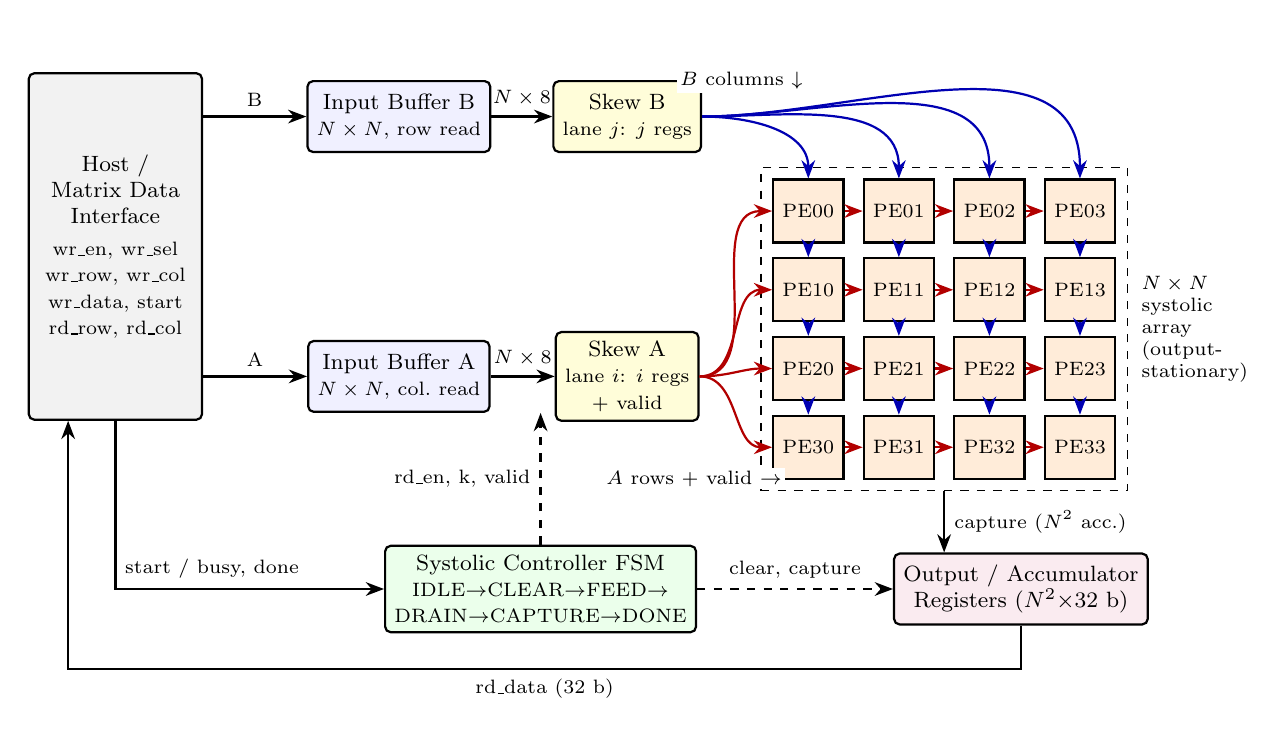
\begin{tikzpicture}[
  font=\footnotesize, >=Stealth,
  blk/.style={draw, thick, rounded corners=2pt, align=center, minimum height=9mm, fill=blue!6},
  pe/.style={draw, thick, minimum size=8mm, fill=orange!15, font=\scriptsize},
  ctl/.style={draw, thick, rounded corners=2pt, align=center, fill=green!8, minimum height=9mm},
  bus/.style={->, thick}]
% host
\node[blk, minimum width=22mm, minimum height=44mm, fill=gray!10] (host) at (0,0.75)
  {Host /\\ Matrix Data\\ Interface\\[2pt]\scriptsize wr\_en, wr\_sel\\\scriptsize wr\_row, wr\_col\\\scriptsize wr\_data, start\\\scriptsize rd\_row, rd\_col};
% buffers
\node[blk, minimum width=22mm] (bufA) at (3.6,-0.9) {Input Buffer A\\\scriptsize $N\times N$, col.\ read};
\node[blk, minimum width=22mm] (bufB) at (3.6, 2.4) {Input Buffer B\\\scriptsize $N\times N$, row read};
\node[blk, minimum width=16mm, fill=yellow!15] (skA) at (6.5,-0.9) {Skew A\\\scriptsize lane $i$: $i$ regs\\\scriptsize + valid};
\node[blk, minimum width=16mm, fill=yellow!15] (skB) at (6.5, 2.4) {Skew B\\\scriptsize lane $j$: $j$ regs};
% PE grid
\foreach \i in {0,...,3}{
 \foreach \j in {0,...,3}{
   \node[pe] (p\i\j) at (8.8+\j*1.15, 1.2-\i*1.0) {PE\i\j};
 }}
\foreach \i in {0,...,3}{
 \foreach \j [count=\jn from 1] in {0,...,2}{ \draw[->, thick, red!70!black] (p\i\j) -- (p\i\jn); }}
\foreach \j in {0,...,3}{
 \foreach \i [count=\in from 1] in {0,...,2}{ \draw[->, thick, blue!70!black] (p\i\j) -- (p\in\j); }}
\node[draw, dashed, inner sep=4pt, fit=(p00)(p33)] (arr) {};
\node[font=\scriptsize, anchor=west] at ($(arr.east)+(0.05,0)$) {\begin{tabular}{@{}l@{}}$N\times N$\\systolic\\array\\(output-\\stationary)\end{tabular}};
% skew to grid (arrows also labeled for grayscale printing)
\node[font=\scriptsize, fill=white, inner sep=1pt] at (7.35,-2.2) {$A$ rows + valid $\rightarrow$};
\node[font=\scriptsize, fill=white, inner sep=1pt] at (7.95,2.85) {$B$ columns $\downarrow$};

\foreach \i in {0,...,3}{ \draw[->, thick, red!70!black] (skA.east) to[out=0,in=180] (p\i0.west); }
\foreach \j in {0,...,3}{ \draw[->, thick, blue!70!black] (skB.east) to[out=0,in=90] (p0\j.north); }
% output
\node[blk, minimum width=24mm, fill=purple!8] (out) at (11.5,-3.6) {Output / Accumulator\\Registers ($N^2\times$32 b)};
\draw[bus] (arr.south) -- node[right,font=\scriptsize]{capture ($N^2$ acc.)} (arr.south |- out.north);
% controller
\node[ctl, minimum width=26mm] (ctl) at (5.4,-3.6) {Systolic Controller FSM\\\scriptsize IDLE$\to$CLEAR$\to$FEED$\to$\\\scriptsize DRAIN$\to$CAPTURE$\to$DONE};
% wiring
\draw[bus] (host.east |- bufA.west) -- node[above,font=\scriptsize]{A} (bufA.west);
\draw[bus] (host.east |- bufB.west) -- node[above,font=\scriptsize]{B} (bufB.west);
\draw[bus] (bufA) -- node[above,font=\scriptsize]{$N\times8$} (skA);
\draw[bus] (bufB) -- node[above,font=\scriptsize]{$N\times8$} (skB);
\draw[bus] (host.south) |- node[pos=0.68,above,font=\scriptsize]{start / busy, done} (ctl.west);
\draw[bus, dashed] (ctl.north) -- node[left,font=\scriptsize]{rd\_en, k, valid} (bufA.south -| ctl.north);
\draw[bus, dashed] (ctl.east) -- node[above,font=\scriptsize]{clear, capture} (out.west);
\draw[bus] (out.south) -- ++(0,-0.55) -| node[pos=0.25,below,font=\scriptsize]{rd\_data (32 b)} ($(host.south)+(-0.6,0)$);
\end{tikzpicture}
\caption{Top-level block diagram of the systolic-array accelerator (shown for $N=4$). $A$ rows and the valid flag enter from the left and move east along the horizontal arrows; $B$ columns enter from the top and move south along the vertical arrows.}
\label{fig:block}
\end{figure*}

\subsection{Output-Stationary Dataflow and Operand Skew}\label{sec:dataflow}
In the OS dataflow, PE$(i,j)$ computes
$C_{ij}=\sum_{k=0}^{N-1}A_{ik}B_{kj}$. Row $i$ of $A$ enters the west edge of
row $i$ and moves one PE east per cycle; column $j$ of $B$ enters the north
edge of column $j$ and moves one PE south per cycle. Let slice $k$ (column $k$
of $A$ and row $k$ of $B$) be read from the buffers in cycle $k$. Lane $i$ of
the A skew buffer delays its operand by $i$ cycles and each PE hop adds one
register, so $A_{ik}$ reaches PE$(i,j)$ at
\begin{equation}
t_A(i,j,k) = k + 1 + i + j ,\label{eq:skew}
\end{equation}
where the $+1$ is the buffer read register. Symmetrically, $B_{kj}$ is delayed
$j$ cycles by its skew lane and travels $i$ hops south, giving
$t_B(i,j,k)=k+1+j+i=t_A(i,j,k)$. Hence \emph{both operands of every product
meet in the correct PE in the same cycle}, which is the fundamental systolic
invariant. The waveform in Fig.~\ref{fig:wave} shows this diagonal wavefront.

\subsection{MAC Unit and Processing Element}
The \texttt{mac\_unit} (Fig.~\ref{fig:pe}) multiplies two signed 8-bit
operands into a 16-bit product, sign-extends it to 32 bits and adds it to the
accumulator when \texttt{en} is high; \texttt{clear} has priority and zeroes
the accumulator. With $|a|,|b|\le128$, each product is at most $2^{14}$, so a
32-bit accumulator cannot overflow for any $N<2^{17}$. Interpreted as Q3.4
fixed-point (value $=x/16$, range $[-8, 7.9375]$), the result is exact in Q7.8
format.

The \texttt{pe} instantiates one MAC and three forwarding registers
(\texttt{a\_out}, \texttt{b\_out}, \texttt{v\_out}). The valid bit travels with
$A$, so a PE accumulates only when real data are present; this makes the
array robust to the zero padding that the skew creates.

\textbf{Pipelined variant (\texttt{PIPE=1}).} Place-and-route showed that the
critical path runs from the PE input registers through the multiplier into
the 32-bit carry chain. Setting \texttt{PIPE=1} inserts a product register
(mapping to the DSP's internal M-register), splitting the path into two
stages at the cost of one cycle of latency.

\begin{figure}[t]
\centering
\resizebox{0.85\columnwidth}{!}{%
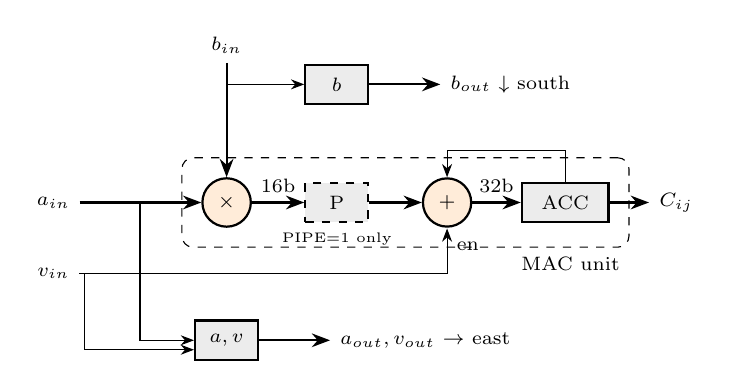
\begin{tikzpicture}[font=\scriptsize, >=Stealth,
  reg/.style={draw, thick, fill=gray!15, minimum width=8mm, minimum height=5mm},
  op/.style={draw, thick, circle, minimum size=6mm, fill=orange!15}]
% MAC datapath
\node[op] (mul) at (1.6,0) {$\times$};
\node[reg, dashed] (preg) at (3.0,0) {P};
\node[op] (add) at (4.4,0) {$+$};
\node[reg, minimum width=11mm] (acc) at (5.9,0) {ACC};
\node[draw, dashed, rounded corners, fit=(mul)(preg)(add)(acc), inner sep=7pt] (mac) {};
\node[font=\scriptsize, anchor=north east] at (mac.south east) {MAC unit};
\node[font=\tiny, below=0pt of preg] {PIPE=1 only};
% inputs
\node (ain) at (-0.6,0) {$a_{in}$};
\node (bin) at (1.6,2.0) {$b_{in}$};
\node (vin) at (-0.6,-0.9) {$v_{in}$};
\draw[->, thick] (ain) -- (mul);
\draw[->, thick] (bin) -- (mul);
\draw[->] (vin) -| node[pos=0.8,right]{en} (4.4,-0.33);
\draw[->, thick] (mul) -- node[above]{16b} (preg);
\draw[->, thick] (preg) -- (add);
\draw[->, thick] (add) -- node[above]{32b} (acc);
\draw[->] (acc.north) -- ++(0,0.4) -| (add.north);
\draw[->, thick] (acc.east) -- ++(0.5,0) node[right]{$C_{ij}$};
% forwarding registers
\node[reg] (ra) at (1.6,-1.75) {$a,v$};
\node[reg] (rb) at (3.0, 1.5) {$b$};
\draw[->] (0.5,0) |- (ra.west);
\draw[->] (-0.2,-0.9) |- ($(ra.west)+(0,-0.12)$);
\draw[->, thick] (ra.east) -- ++(0.9,0) node[right]{$a_{out}, v_{out}$ $\rightarrow$ east};
\draw[->] (1.6,1.5) -- (rb.west);
\draw[->, thick] (rb.east) -- ++(0.9,0) node[right]{$b_{out}$ $\downarrow$ south};
\end{tikzpicture}}
\caption{Processing element micro-architecture. The dashed product register is present only in the pipelined variant.}
\label{fig:pe}
\end{figure}

\subsection{Input, Skew and Output Buffers}
Each \texttt{input\_buffer} stores an $N\times N$ matrix addressed by the
concatenation \{row, col\}. Using a power-of-two stride instead of
$\textit{row}\cdot N+\textit{col}$ removed an address multiplier that the
synthesizer otherwise mapped into a DSP block for $N=3$, reducing the
$3\times3$ ECP5 LUT count from 1\,913 to 764. Buffer A reads a column per
cycle and buffer B a row per cycle. The \texttt{skew\_buffer} is a
triangular shift register (lane $i$ has $i$ stages, $N(N-1)/2$ stages in
total). The \texttt{output\_buffer} captures all $N^2$ accumulators in one
cycle and exposes them through a two-level (row, column) read multiplexer.

\subsection{Controller}
The controller finite-state machine (FSM) is shown in Fig.~\ref{fig:fsm} and Table~\ref{tab:fsm}.
The drain length follows from \eqref{eq:skew}: the final product ($i=j=k=N-1$) is
accumulated at $t=3N-2$ counted from the first FEED cycle, i.e.\ $2N-1$ cycles
after the last FEED cycle. We verified that this is minimal: with a drain of
$2N-2$ cycles the system testbench fails because PE$(N-1,N-1)$ is captured one
cycle too early. Summing the states,
\begin{equation}
\begin{aligned}
L_{\text{sys}} &= \underbrace{1}_{\text{CLR}} + \underbrace{N}_{\text{FEED}} + \underbrace{2N-1+P}_{\text{DRAIN}} + \underbrace{1}_{\text{CAPT}}\\
&= 3N+1+P
\end{aligned}\label{eq:lsys}
\end{equation}
cycles, where $P\in\{0,1\}$ is the \texttt{PIPE} parameter.

\begin{figure}[t]
\centering
\resizebox{0.85\columnwidth}{!}{%
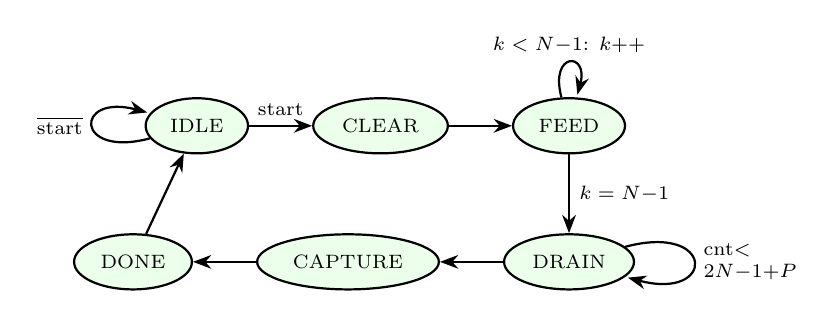
\begin{tikzpicture}[font=\scriptsize, >=Stealth, node distance=10mm and 8mm,
  st/.style={draw, thick, ellipse, minimum width=13mm, minimum height=7mm, fill=green!8}]
\node[st] (idle) {IDLE};
\node[st, right=of idle] (clr) {CLEAR};
\node[st, right=of clr] (feed) {FEED};
\node[st, below=of feed] (drain) {DRAIN};
\node[st, left=of drain] (cap) {CAPTURE};
\node[st, left=of cap] (done) {DONE};
\draw[->, thick] (idle) -- node[above]{start} (clr);
\draw[->, thick] (clr) -- (feed);
\draw[->, thick] (feed) edge[loop above] node{$k<N{-}1$: $k{+}{+}$} (feed);
\draw[->, thick] (feed) -- node[right]{$k=N{-}1$} (drain);
\draw[->, thick] (drain) edge[loop right] node[align=left]{cnt$<$\\$2N{-}1{+}P$} (drain);
\draw[->, thick] (drain) -- (cap);
\draw[->, thick] (cap) -- (done);
\draw[->, thick] (done) -- (idle);
\draw[->, thick] (idle) edge[loop left] node{$\overline{\text{start}}$} (idle);
\end{tikzpicture}}
\caption{State-transition diagram of the systolic controller.}
\label{fig:fsm}
\end{figure}

\begin{table}[t]
\centering
\caption{Controller states and outputs}
\label{tab:fsm}
\setlength{\tabcolsep}{3pt}
\begin{tabular}{@{}lcl@{}}
\toprule
State & Cycles & Action \\
\midrule
IDLE    & --        & wait for \texttt{start}; buffers writable \\
CLEAR   & 1         & \texttt{clear}=1: zero accumulators \& pipeline regs \\
FEED    & $N$       & \texttt{rd\_en}=1, \texttt{rd\_k}$=0\ldots N{-}1$ \\
DRAIN   & $2N{-}1{+}P$ & wait for wavefront to reach PE$(N{-}1,N{-}1)$ \\
CAPTURE & 1         & \texttt{capture}=1: copy $N^2$ results \\
DONE    & 1         & \texttt{done} pulse, \texttt{busy}=0 \\
\bottomrule
\end{tabular}
\end{table}

\subsection{Baseline: Sequential Single-MAC Multiplier}
For comparison, \texttt{sequential\_matmul} has the identical host interface
but a single \texttt{mac\_unit} executing the $i,j,k$ triple loop: $N$ MAC
cycles plus one write-back cycle per output element, i.e.
\begin{equation}
L_{\text{seq}} = N^2(N+1)+1 .\label{eq:lseq}
\end{equation}

\subsection{Module Hierarchy and FPGA Demonstrator}
The hierarchy is \texttt{systolic\_top} $\supset$ \{\texttt{systolic\_controller},
2$\times$\texttt{input\_buffer}, 2$\times$\texttt{skew\_buffer},
\texttt{systolic\_array} $\supset N^2\times$\texttt{pe} $\supset$
\texttt{mac\_unit}, \texttt{output\_buffer}\}. A \texttt{basys3\_demo\_top}
wrapper loads one of two demo matrix pairs from a ROM after reset, starts the
accelerator from push-button \texttt{btnC}, selects $C_{ij}$ with four slide
switches and displays it in hexadecimal on the 7-segment display; LEDs show the
\texttt{done} flag and the measured cycle count.

% ============================================================================
\section{Verification}

\subsection{Methodology}
Verification followed the bottom-up workflow of the brief: one PE, then the
array, then the system. All testbenches are self-checking and print a
PASS/FAIL verdict; simulation used Icarus Verilog~13 with
\texttt{-Wall} (zero warnings)~\cite{icarus} and value change dump (VCD)
files for waveform inspection.
\begin{itemize}\setlength{\itemsep}{1pt}
\item \textbf{\texttt{tb\_mac\_unit}} (74 checks): sign combinations, zero
  operand, \texttt{en}=0 hold, $127^2$, $(-128)^2$, $-128\cdot127$, clear
  priority and a 64-term accumulation of $(-128)^2$ (=1\,048\,576).
\item \textbf{\texttt{tb\_pe}} (14 checks): one-cycle forwarding of $a$, $b$
  and valid, no accumulation when invalid, clear, and an 8-term dot product.
\item \textbf{\texttt{tb\_systolic\_top}} (112 products per $N$): identity,
  zero, all-ones, worked example, mixed signs, extreme values $(-128)$ and
  $127\times-128$, diagonal, Q3.4 fixed-point, three back-to-back jobs and 100
  random matrix pairs; results compared with an in-testbench reference model
  and logged for an independent NumPy check.
\item \textbf{\texttt{tb\_compare}}: identical random inputs to the systolic
  and sequential designs for $N\in\{2,3,4,5,6,8\}$ with and without
  \texttt{PIPE}; checks agreement and records latency.
\item \textbf{\texttt{tb\_fpga\_demo}}: smoke test of the Basys-3 wrapper.
\end{itemize}

\subsection{Results}
Every testbench passed. Table~\ref{tab:verif} summarizes the coverage. The
NumPy~\cite{numpy} model (\texttt{verify\_results.py}) re-computed all 224 logged products
and found zero mismatches; for the Q3.4 test the maximum error against
floating-point $A\cdot B$ was exactly 0, confirming that the fixed-point path
is lossless. For the worked example ($A=1..16$, $B=16..1$ row-major) the array
returns $C_{00}=80$, $C_{12}=188$ and $C_{33}=386$, matching the reference.

\begin{table}[t]
\centering
\caption{Verification summary (all passed)}
\label{tab:verif}
\setlength{\tabcolsep}{4pt}
\begin{tabular}{@{}lrrc@{}}
\toprule
Testbench & Tests & Elements & Result\\
\midrule
\texttt{tb\_mac\_unit}            & 74  & --    & PASS\\
\texttt{tb\_pe}                   & 14  & --    & PASS\\
\texttt{tb\_systolic\_top} $N{=}3$ & 112 & 1\,008 & PASS\\
\texttt{tb\_systolic\_top} $N{=}4$ & 112 & 1\,792 & PASS\\
\texttt{tb\_systolic\_top} $N{=}4$, PIPE & 112 & 1\,792 & PASS\\
\texttt{tb\_compare} $N{=}2..8$ ($\times2$) & 240 & 6\,160 & PASS\\
NumPy golden model                & 224 & 2\,800 & 0 mismatches\\
\bottomrule
\end{tabular}
\end{table}

\begin{figure*}[t]
\centering
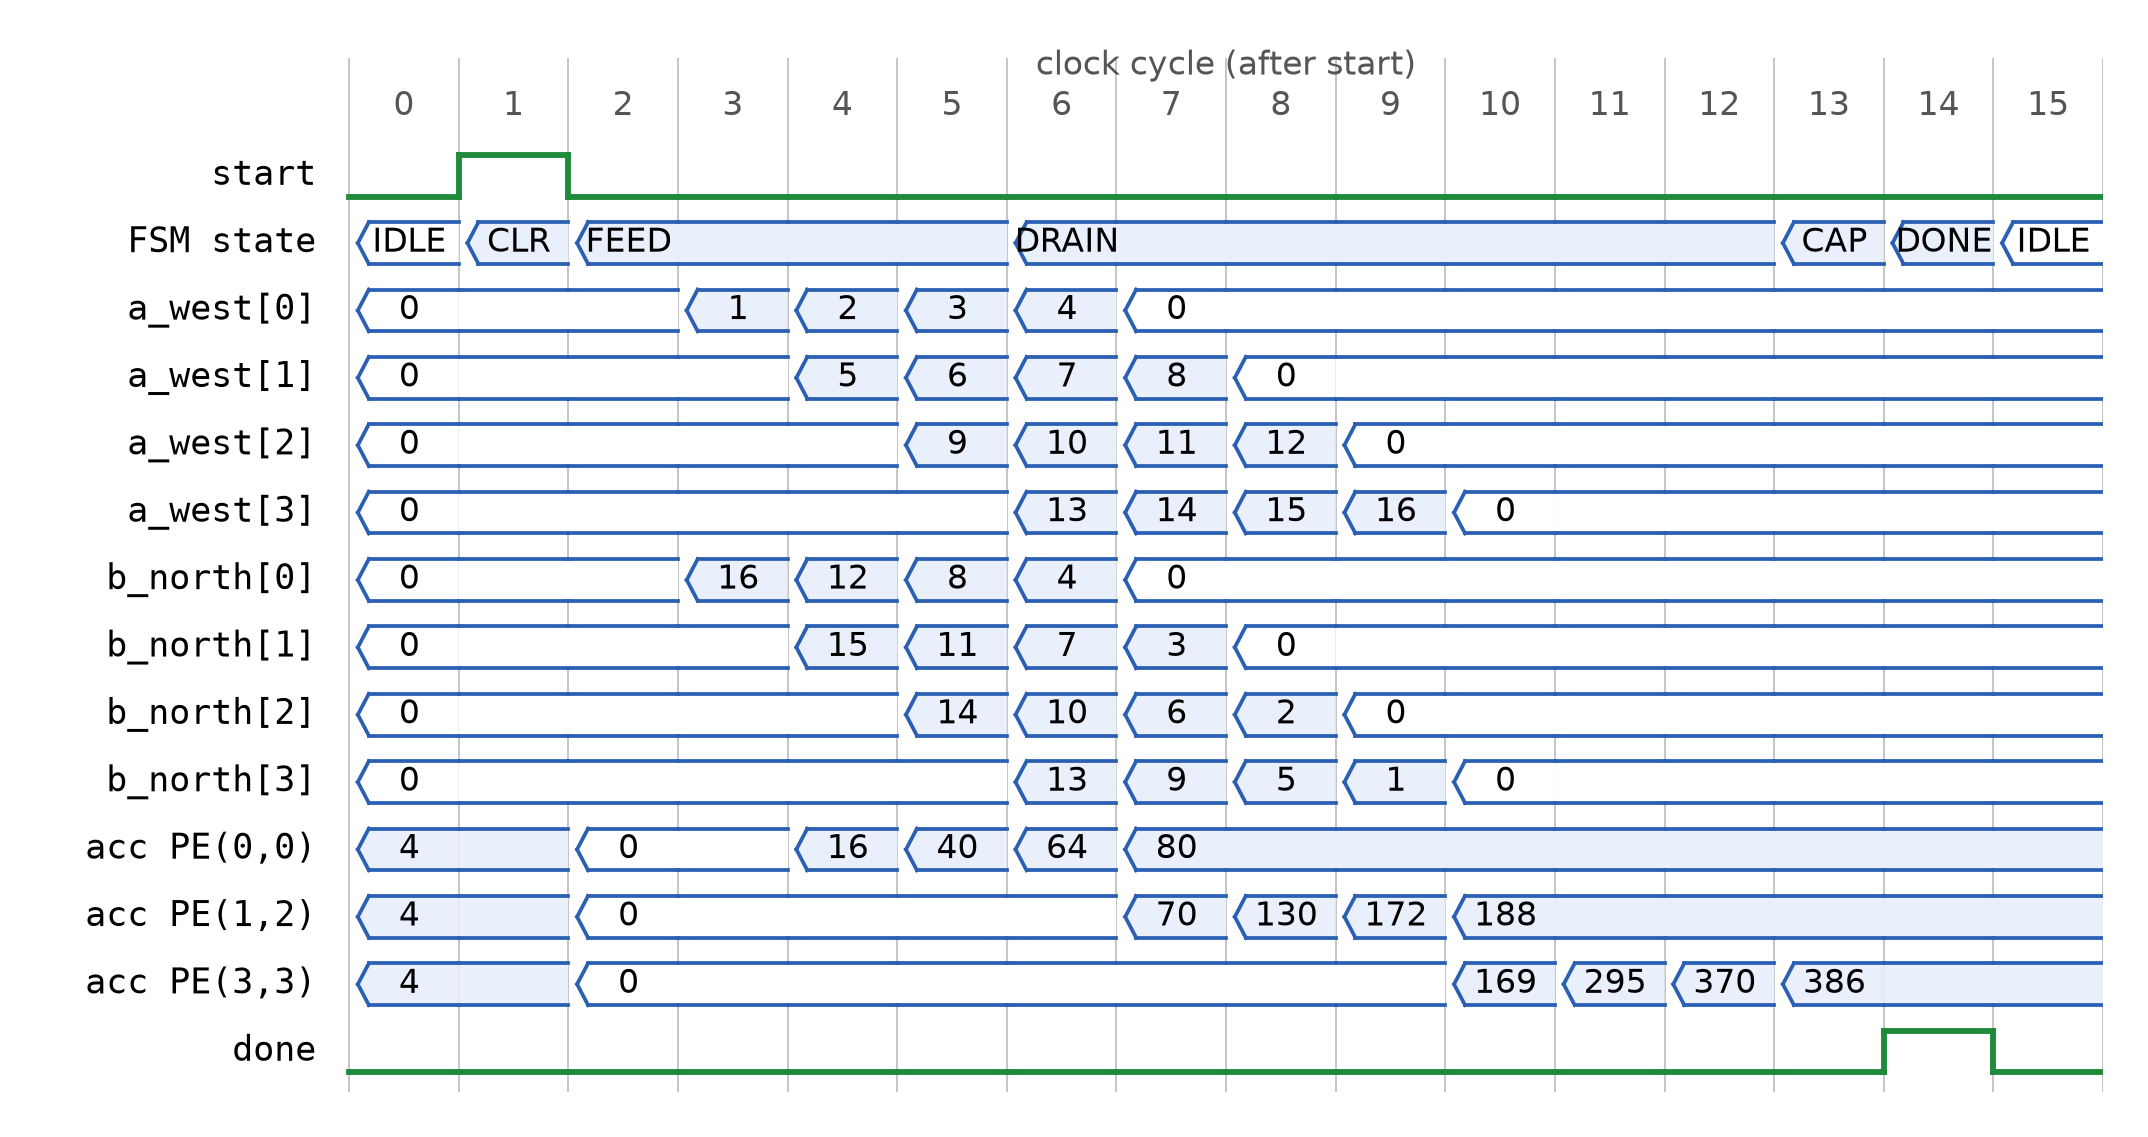
\includegraphics[width=0.92\textwidth]{waveform_worked_example.png}
\caption{Simulation waveform (rendered from the VCD) of the worked example on the $4\times4$ array. Row $i$ of $A$ and column $j$ of $B$ enter $i$ (resp.\ $j$) cycles late, producing the diagonal wavefront; PE(0,0) holds its final value from cycle 7, PE(1,2) from cycle 10 and PE(3,3) from cycle 13; \texttt{done} is asserted $3N+1=13$ cycles after \texttt{start} is sampled.}
\label{fig:wave}
\end{figure*}

% ============================================================================
\section{Performance and Implementation Results}

\subsection{Latency and Throughput}
Table~\ref{tab:cycles} lists the measured start-to-done latencies. They match
\eqref{eq:lsys} and \eqref{eq:lseq} exactly for every $N$. The systolic latency is linear in
$N$ while the baseline is cubic, so the cycle speed-up grows as
\begin{equation}
S(N)=\frac{N^2(N+1)+1}{3N+1}\approx\frac{N^2}{3},
\end{equation}
reaching $23.1\times$ for $N=8$ (Fig.~\ref{fig:speedup}). Throughput in MACs
per cycle is $N^3/(3N+1)$ for one isolated job, approaching the peak of $N^2$
MAC/cycle only if successive jobs are overlapped (Section~\ref{sec:disc}).

\begin{table}[t]
\centering
\caption{Measured latency (cycles) for one $N\times N$ product}
\label{tab:cycles}
\setlength{\tabcolsep}{4pt}
\begin{tabular}{@{}rrrrrr@{}}
\toprule
$N$ & MACs & Systolic & Sys.\ (PIPE) & Sequential & Speed-up\\
\midrule
2 & 8   & 7  & 8  & 13  & 1.86$\times$\\
3 & 27  & 10 & 11 & 37  & 3.70$\times$\\
\textbf{4} & 64 & \textbf{13} & 14 & \textbf{81} & \textbf{6.23$\times$}\\
5 & 125 & 16 & 17 & 151 & 9.44$\times$\\
6 & 216 & 19 & 20 & 253 & 13.32$\times$\\
8 & 512 & 25 & 26 & 577 & 23.08$\times$\\
\bottomrule
\end{tabular}
\end{table}

\begin{figure*}[t]
\centering
\includegraphics[width=0.325\textwidth]{latency_vs_N.png}\hfill
\includegraphics[width=0.325\textwidth]{speedup_vs_N.png}\hfill
\includegraphics[width=0.325\textwidth]{throughput_vs_N.png}
\caption{Measured results versus matrix size: latency in cycles (left, log scale), cycle speed-up over the sequential baseline (center) and throughput in MACs per cycle (right).}
\label{fig:speedup}\label{fig:thr}
\end{figure*}

\subsection{Resource Utilization and Timing}
The RTL was synthesized with Yosys~\cite{yosys} for the Xilinx Artix-7
(\texttt{synth\_xilinx}) and for the Lattice ECP5-25F, which was then placed
and routed with nextpnr~\cite{shah2019yosys} to obtain a post-route maximum
frequency. A Vivado batch script and Basys-3 constraints are provided to
reproduce the Xilinx flow. Results are in Table~\ref{tab:res}.

\begin{table*}[t]
\centering
\caption{Synthesis and place-and-route results}
\label{tab:res}
\begin{tabular}{@{}lrrrrrrrr@{}}
\toprule
& \multicolumn{4}{c}{Xilinx Artix-7 (Yosys)} & \multicolumn{4}{c}{Lattice ECP5-25F (Yosys + nextpnr, post-route)}\\
\cmidrule(lr){2-5}\cmidrule(l){6-9}
Design & LUT & LUTRAM & FF & DSP48E1 & LUT4 & FF & MULT18 & $F_{\max}$ (MHz)\\
\midrule
Systolic $3\times3$                 & 173 & 40 & 430 & 9  & 764   & 814   & 9  & 98.97\\
Systolic $4\times4$                 & 233 & 64 & 789 & 16 & 1\,129 & 1\,429 & 16 & 100.50\\
Systolic $4\times4$, pipelined MAC  & 230 & 64 & 793 & 16 & 1\,141 & 1\,689 & 16 & \textbf{127.02}\\
Sequential 1-MAC, $N=3$             & 37  & 40 & 28  & 1  & 160   & 60    & 1  & 95.13\\
Sequential 1-MAC, $N=4$             & 35  & 40 & 28  & 1  & 161   & 60    & 1  & 92.66\\
\bottomrule
\end{tabular}
\end{table*}

On Artix-7 each MAC (multiplier, 32-bit adder and accumulator register) is
absorbed entirely into one DSP48E1 slice~\cite{xilinx2018dsp48}, which is why
the 4$\times$4 array needs only 233 LUTs and 789 flip-flops (FFs) (mostly operand,
skew and output registers). ECP5's MULT18X18D has no post-adder in this
mapping, so the accumulators and carry chains are built in fabric, raising
LUT4 and FF counts. The DSP count scales as $N^2$ and is the resource that
limits array size: the ECP5-25F (28 multipliers) fits up to $5\times5$,
whereas a Basys-3 xc7a35t (90 DSP48E1) fits up to $9\times9$.

\subsection{Comparison with the Baseline}
Table~\ref{tab:wall} converts cycles to time at each design's own post-route
$F_{\max}$. The $4\times4$ array completes a product in 129.4\,ns (110.2\,ns
pipelined) against 874.2\,ns for the baseline: a $6.8\times$ ($7.9\times$)
wall-clock speed-up, delivering 1.16\,GOPS (1\,MAC = 2\,ops) with 16 multipliers.
Per multiplier the array is about half as efficient as the baseline
(0.073 vs.\ 0.146\,GOPS/DSP) because the isolated-job latency includes
$2N-1$ fill/drain cycles in which most PEs idle; this is the classic
systolic utilization cost, discussed next.

\begin{table}[t]
\centering
\caption{Wall-clock comparison at post-route $F_{\max}$ (ECP5)}
\label{tab:wall}
\setlength{\tabcolsep}{3pt}
\begin{tabular}{@{}lrrrr@{}}
\toprule
Design ($N=4$) & Cycles & $F_{\max}$ & Latency & GOPS\\
\midrule
Sequential 1-MAC     & 81 & 92.66  & 874.2\,ns & 0.146\\
Systolic             & 13 & 100.50 & 129.4\,ns & 0.990\\
Systolic, pipelined  & 14 & 127.02 & 110.2\,ns & 1.161\\
\midrule
Speed-up (pipelined vs.\ seq.) & \multicolumn{4}{r}{$7.93\times$ latency, $7.95\times$ throughput}\\
\bottomrule
\end{tabular}
\end{table}

\subsection{Discussion}\label{sec:disc}
\textbf{Pipelining trade-off.} Registering the product adds one cycle
($13\to14$) but raises $F_{\max}$ by 26\% ($100.5\to127.0$\,MHz), a net
15\% latency reduction---a direct application of the pipelining principle
of the course: deeper pipelines trade latency in cycles for a shorter clock
period.

\textbf{PE utilization.} During one job each PE is busy for $N$ of the
$3N+1$ cycles (31\% for $N=4$). Because the controller can accept a new
\texttt{start} as soon as the previous results are captured, and because
the output registers decouple read-out from computation, the array could be
extended with double-buffered accumulators so that job $m+1$ is fed while job
$m$ drains, achieving one product every $N$ cycles and the peak $N^2$
MAC/cycle (Fig.~\ref{fig:thr}).

\textbf{I/O bound (Amdahl's law).} The demonstration interface writes one
8-bit element per cycle, so loading $A$ and $B$ costs $2N^2=32$ cycles and
reading $C$ costs $N^2=16$ cycles for $N=4$. End-to-end, the systolic
design takes $32+13+16=61$ cycles against $32+81+16=129$, a $2.1\times$
speed-up. Exactly as Kung argued~\cite{kung1982why}, a systolic array is only
as fast as the bandwidth that feeds it; real accelerators use wide on-chip
static random-access memory (SRAM) buffers and direct memory access (DMA) (TPU's 24\,MiB unified buffer~\cite{jouppi2017tpu}).


\textbf{Limitations and future work.} (i) Matrices larger than $N\times N$
require tiling in software or a tiling controller; (ii) the accumulator is not
saturated or re-quantized back to 8 bits; (iii) a weight-stationary mode as
in Gemmini~\cite{genc2021gemmini} and an AXI-Stream interface would make the
design usable as a real SoC peripheral.

% ============================================================================
\section{Conclusion}
We designed, verified and implemented a parameterized output-stationary
systolic-array accelerator for INT8/Q3.4 fixed-point matrix multiplication.
The design follows the brief's workflow---one PE, then the array, then
streaming and verification against a reference model---and exhibits exactly
the predicted $3N+1$-cycle latency. On FPGA, the $4\times4$ array runs at
up to 127\,MHz and computes a matrix product $7.9\times$ faster than a
single-MAC sequential baseline, while the analysis shows how fill/drain
overhead and I/O bandwidth bound real-world speed-up---the same trade-offs
that shape commercial AI accelerators.

% ============================================================================
\section*{Individual Contributions}
{\small
\begin{tabular}{@{}>{\raggedright\arraybackslash}p{0.34\columnwidth}>{\raggedright\arraybackslash}p{0.57\columnwidth}@{}}
\toprule
Member (Enrollment No.) & Contribution\\
\midrule
Syed Darain Qamar\newline(2401010472) & Team lead; architecture and dataflow; \texttt{systolic\_array} and \texttt{systolic\_top}; latency model.\\
Md Sajjan\newline(2401010272) & \texttt{mac\_unit} and \texttt{pe}; fixed-point format; pipelined MAC; unit testbenches.\\
Sibtain Ahmed Qureshi\newline(2401010454) & Controller FSM; input, skew and output buffers; data interface.\\
Abuzar Haideri\newline(2401010024) & System and comparison testbenches; reference and NumPy models; waveforms.\\
Antik Mondal\newline(2401010084) & Sequential baseline; synthesis and place-and-route; Basys-3 demo; performance analysis.\\
\bottomrule
\end{tabular}}

% ============================================================================
\begin{thebibliography}{99}

\bibitem{kung1979systolic}
H.~T. Kung and C.~E. Leiserson, ``Systolic arrays (for VLSI),'' in
\emph{Sparse Matrix Proceedings 1978}. Philadelphia, PA, USA: SIAM, 1979,
pp.~256--282.

\bibitem{kung1982why}
H.~T. Kung, ``Why systolic architectures?'' \emph{Computer}, vol.~15, no.~1,
pp.~37--46, Jan. 1982.

\bibitem{jouppi2017tpu}
N.~P. Jouppi \emph{et al.}, ``In-datacenter performance analysis of a tensor
processing unit,'' in \emph{Proc. 44th Annu. Int. Symp. Comput. Archit.
(ISCA)}, Toronto, ON, Canada, 2017, pp.~1--12.

\bibitem{hennessy2019ca}
J.~L. Hennessy and D.~A. Patterson, \emph{Computer Architecture: A
Quantitative Approach}, 6th~ed. Cambridge, MA, USA: Morgan Kaufmann, 2019.

\bibitem{kung1988vlsi}
S.~Y. Kung, \emph{VLSI Array Processors}. Englewood Cliffs, NJ, USA:
Prentice Hall, 1988.

\bibitem{chen2017eyeriss}
Y.-H. Chen, T.~Krishna, J.~S. Emer, and V.~Sze, ``Eyeriss: An
energy-efficient reconfigurable accelerator for deep convolutional neural
networks,'' \emph{IEEE J. Solid-State Circuits}, vol.~52, no.~1,
pp.~127--138, Jan. 2017.

\bibitem{sze2017efficient}
V.~Sze, Y.-H. Chen, T.-J. Yang, and J.~S. Emer, ``Efficient processing of deep
neural networks: A tutorial and survey,'' \emph{Proc. IEEE}, vol.~105,
no.~12, pp.~2295--2329, Dec. 2017.

\bibitem{du2015shidiannao}
Z.~Du \emph{et al.}, ``ShiDianNao: Shifting vision processing closer to the
sensor,'' in \emph{Proc. 42nd Annu. Int. Symp. Comput. Archit. (ISCA)},
2015, pp.~92--104.

\bibitem{genc2021gemmini}
H.~Genc \emph{et al.}, ``Gemmini: Enabling systematic deep-learning
architecture evaluation via full-stack integration,'' in \emph{Proc. 58th
ACM/IEEE Design Autom. Conf. (DAC)}, 2021, pp.~769--774.

\bibitem{samajdar2018scalesim}
A.~Samajdar, Y.~Zhu, P.~Whatmough, M.~Mattina, and T.~Krishna, ``SCALE-Sim:
Systolic CNN accelerator simulator,'' \emph{arXiv:1811.02883}, 2018.

\bibitem{jacob2018quantization}
B.~Jacob \emph{et al.}, ``Quantization and training of neural networks for
efficient integer-arithmetic-only inference,'' in \emph{Proc. IEEE/CVF Conf.
Comput. Vis. Pattern Recognit. (CVPR)}, 2018, pp.~2704--2713.

\bibitem{xilinx2018dsp48}
Xilinx Inc., ``7 Series DSP48E1 Slice User Guide,'' UG479 (v1.10), Mar. 2018.

\bibitem{patterson2020cod}
D.~A. Patterson and J.~L. Hennessy, \emph{Computer Organization and Design
RISC-V Edition: The Hardware/Software Interface}, 2nd~ed. Cambridge, MA,
USA: Morgan Kaufmann, 2020.

\bibitem{icarus}
S.~Williams, ``Icarus Verilog.'' Accessed: Nov. 18, 2026. [Online]. Available:
\url{https://steveicarus.github.io/iverilog/}

\bibitem{numpy}
C.~R. Harris \emph{et al.}, ``Array programming with NumPy,'' \emph{Nature},
vol.~585, no.~7825, pp.~357--362, Sep. 2020.

\bibitem{yosys}
C.~Wolf, ``Yosys Open SYnthesis Suite.'' Accessed: Nov. 18, 2026. [Online].
Available: \url{https://yosyshq.net/yosys/}

\bibitem{shah2019yosys}
D.~Shah \emph{et al.}, ``Yosys+nextpnr: An open source framework from Verilog
to bitstream for commercial FPGAs,'' in \emph{Proc. IEEE 27th Annu. Int. Symp.
Field-Programmable Custom Comput. Mach. (FCCM)}, 2019, pp.~1--4.

\end{thebibliography}

\end{document}
